\documentclass{article}
\usepackage[pdftex]{graphicx,color}
\usepackage[T1]{fontenc}
\usepackage{lmodern}
\usepackage{amsfonts}
\usepackage{subfigure}
\usepackage{textpos}
\usepackage{amsmath,amssymb} 
\usepackage{physics}
\usepackage{fullpage}

% be able to use \note environments with a box around the text
\usepackage{fancybox}
\newcommand{\note}[1]{
{\parindent0pt
  \begin{center}
    \shadowbox{
      \begin{minipage}[c]{0.9\linewidth}
        \textbf{Note:} #1
      \end{minipage}
    }
  \end{center}
}}

% use the listings package for code snippets. define keywords for prm files
% and for gnuplot
\usepackage{listings}
\lstset{
  language=C++,
  showstringspaces=false,
  basicstyle=\small\ttfamily,
  columns=fullflexible,
  keepspaces=true,
  frame=single,
  breaklines=true,
  postbreak=\raisebox{0ex}[0ex][0ex]{\hspace{5em}\ensuremath{\color{red}\hookrightarrow\space}}
}
\lstdefinelanguage{prmfile}{morekeywords={set,subsection,end},
                            morecomment=[l]{\#},escapeinside={\%\%}{\%},}
\lstdefinelanguage{gnuplot}{morekeywords={plot,using,title,with,set,replot},
                            morecomment=[l]{\#},}


% use the hyperref package; set the base for relative links to
% the top-level aspect directory so that we can link to
% files in the aspect tree without having to specify the
% location relative to the directory where the pdf actually
% resides
\usepackage[colorlinks,linkcolor=blue,urlcolor=blue,citecolor=blue,baseurl=../]{hyperref}

\newcommand{\dealii}{{\textsc{deal.II}}}
\newcommand{\pfrst}{{\normalfont\textsc{p4est}}}
\newcommand{\trilinos}{{\textsc{Trilinos}}}
\newcommand{\petsc}{{\textsc{PETSc}}}
\newcommand{\aspect}{\textsc{ASPECT}}

\begin{document}

\begin{center}
\textbf{\large{Viscosity variations for a convective box with aspect}}
\end{center}

\vspace{0.2cm}
\textbf{How to change the viscosity definition}
\vspace{0.2cm}

One way to change the viscosity definition is to define a new class of the MaterialModel, in a ".cc" file. In this exemple, the name of the class is "SimplerWithCrust". Each new parameter that is added has to be declared in order to be read in the parameter file. 
\lstinputlisting[language=prmfile]{cookbooks/convection-box/parametersviscosityjump.prm}
It's necessary to compile in order to have the shared library associated (cmake and make into the folder of the new ".cc" file).

In the input file, this shared librairy has to be called and the new class that has been implemented has to be added in the Material Model subsection, together with  the new parameters that are defined in the ".cc" file :

\lstinputlisting[language=prmfile]{cookbooks/convection-box/materialmodel.prm}

For the moment, three different definitions of the viscosity have been tested (Figure~\ref{convectionbox}) : a constant viscosity (cookbooks/convection-box), a jump of viscosity at a given position (cookbooks/convection-box-viscosity-jump) and a linear viscosity (cookbooks/convection-box-linear-viscosity).

The viscosity jump is defined as :

\lstinputlisting[language=prmfile]{cookbooks/convection-box/definitionviscosityjump.prm}

The linear viscosity is defined as :

\lstinputlisting[language=prmfile]{cookbooks/convection-box/definitionlinearviscosity.prm}

For the viscosity jump, a "high" jump and a "low" jump have been tested (Figure~\ref{viscosityjump}).

\vspace{0.2cm}
\textbf{Some results - Next steps}
\vspace{0.2cm}

Figure~\ref{convectionbox} shows preliminary results with a Rayleigh number of $10^4$ for the differents viscosity definitions that have been tested. Figure~\ref{viscosityjump} shows the difference between a low and a high viscosity jump.

The next steps will be first to look for simulations with higher Rayleigh numbers and thus more complicate plumes. It could also be interessant to compare with a "smooth" definition, in between the linear viscosity and the jump of viscosity. 

\textbf{Solid-state phase transition} (Treatrise on Geophysics -Numerical method for mantle convection, p212). In the long term, it could be good to look at solid state phase transition in the inner core, in order to see the effect on the dynamic. Phase transitions $k$ affect the momentum equation, by adding buoyancy force at the phase boundary. This is called 'phase boundary undulations' and can be described by a dimensionnless phase change function $\Gamma_k$ that varies between 0 to 1, which respectively represent the two phases separated by this phase change boundary. The momentum equation can be written as
 \begin{equation}
\sigma_{ij,j} + \Bigg(Ra T - \sum\limits_{k} Ra_k \Gamma_k\Bigg) \delta_{iz} = 0 
\end{equation}
where phase change Rayleigh number $Ra_k$ is
\begin{equation}
Ra_k= \frac{\Delta \rho_k g D^3}{\kappa \eta_0}
\end{equation}
with $\Delta \rho_k$ the density change.
The phase change function being defined via the 'excess pressure', which depends on the Clapeyron slope $\gamma_k$ and the phase change pressure at zero degree temperature for the $k$th phase transition $P_0$, it will thus be necessary to define a Clapeyron slope adapted for the inner core (in \textit{aspect} the phase change parameters are for the mantle). The nondimensionnal 'excess pressure' can be written as 
\begin{equation}
 \pi_k = 1 - d_k - z - \gamma_k (T - T_k)
\end{equation}
where $\gamma_k, d_k$ and $T_k$ are the nondimensionnal Clapeyron slope, reference phase transition depth, and reference phase transition temperature for the $k$th phase transition, respectively. The dimensionless phase change function is thus given as 
\begin{equation}
 \Gamma_k = \frac{1}{2} \Bigg(1 + tanh \frac{\pi_k}{d}\Bigg)
\end{equation}
where $d$ is dimensionless phase transition width that measures the depth segment over which the phase change occurs.  

The nonlinear energy equation has also to be change, in order to include the latent heating effect along with viscous heating and the adiabatic heating :
\begin{equation}
\Bigg[1 + \sum\limits_{k} \frac{Ra_k d \Gamma_k}{Ra d \pi_k} D_i (T + T_s) \Bigg] \Bigg(\frac{\partial T}{\partial t} + \overrightarrow{v} . \grad T \Bigg) + \Bigg(1 +  \sum\limits_{k}  \gamma_k  \frac{Ra_k d \Gamma_k}{Ra d \pi_k} \Bigg) (T - T_s) D_i v_z = \Delta T + \frac{D_i}{Ra} \tau_{ij} \frac{\partial v_i}{\partial x_j} + \gamma
\end{equation}
where $T_s, v_z$ and $\tau_{ij}$ are the surface temperature, vertical velocity, and deviatoric stress, respectively; $k$ is a phase change index and $D_i$ is the dissipation number defined as 
\begin{equation}
D_i = \frac{\alpha g D}{C_p}.
\end{equation}

Finally, apply all this definitions to a sphere in order to properly model an inner core dynamics with solid-state phase change transition.

\begin{figure}
    \begin{center}
    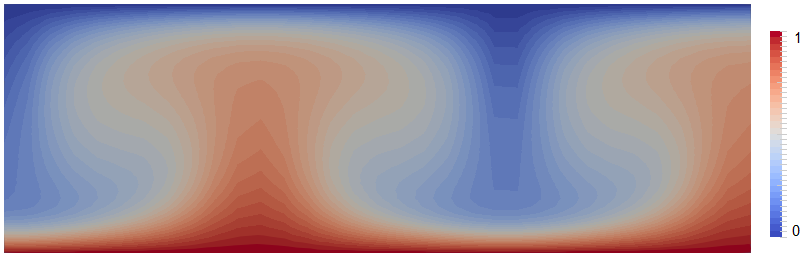
\includegraphics[width=0.55\linewidth]{cookbooks/convection-box/convectionboxratio3modif.png}
    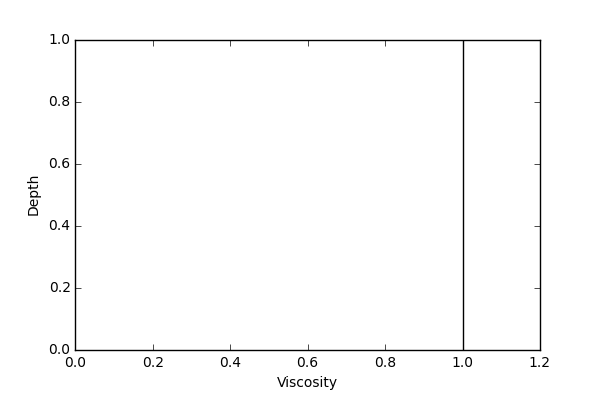
\includegraphics[width=0.2\linewidth]{cookbooks/convection-box/constantviscosityprofile.png}
    
    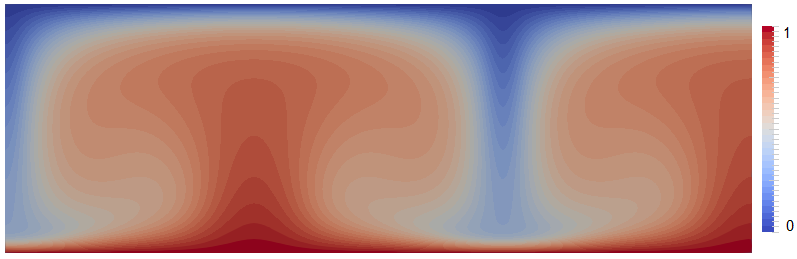
\includegraphics[width=0.55\linewidth]{cookbooks/convection-box/linearviscosityratio3modif.png}
    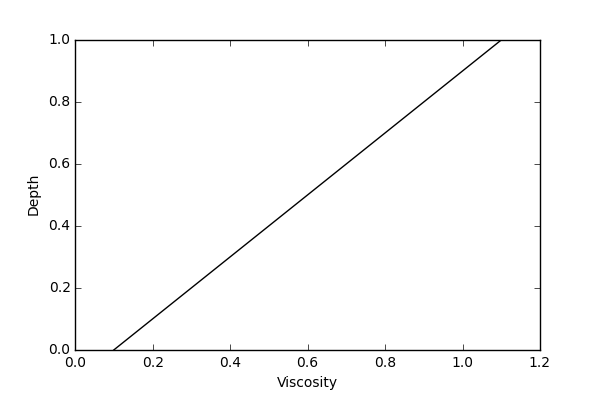
\includegraphics[width=0.2\linewidth]{cookbooks/convection-box/linearviscosityprofile.png}

    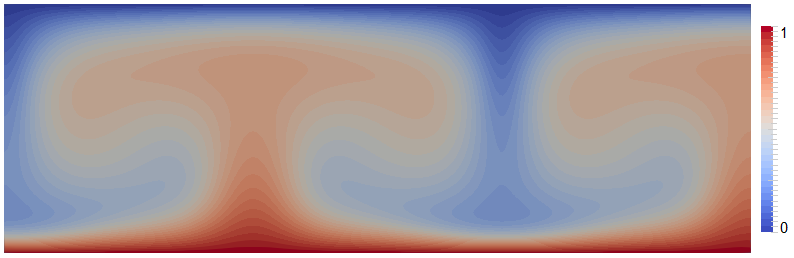
\includegraphics[width=0.55\linewidth]{cookbooks/convection-box/viscosityjumpratio3modif.png}
    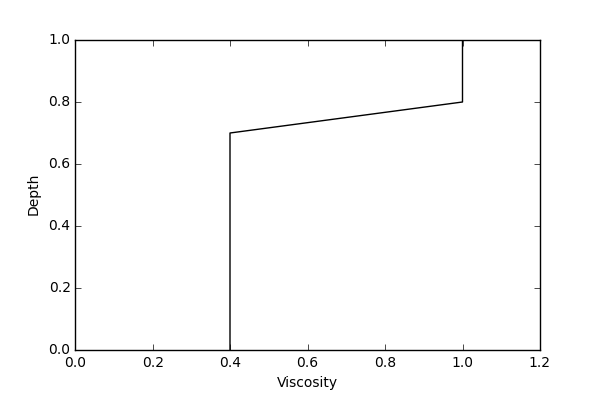
\includegraphics[width=0.2\linewidth]{cookbooks/convection-box/viscosityjumpprofile.png}
    \caption{Convection box and the viscosity profile associated with from the top to the bottom, constant viscosity, linear viscosity and viscosity jump, for $Ra=10^4$.}
    \label{convectionbox}
       \end{center}
\end{figure}

\begin{figure}
    \begin{center}
    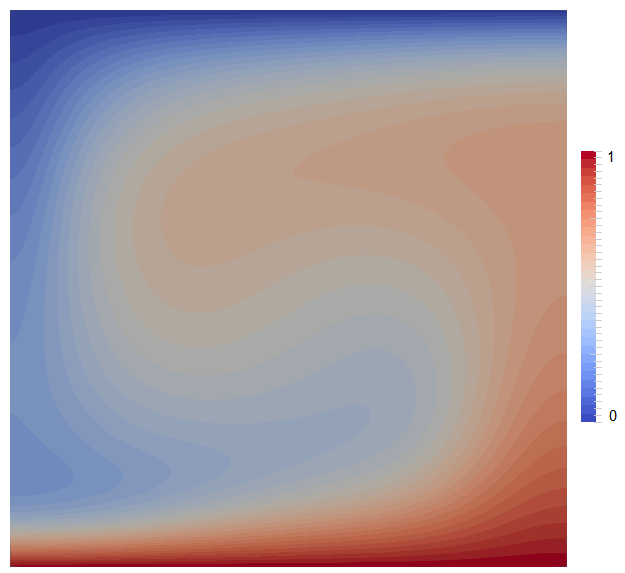
\includegraphics[width=0.3\linewidth]{cookbooks/convection-box/viscosityjumpmodif.png}
    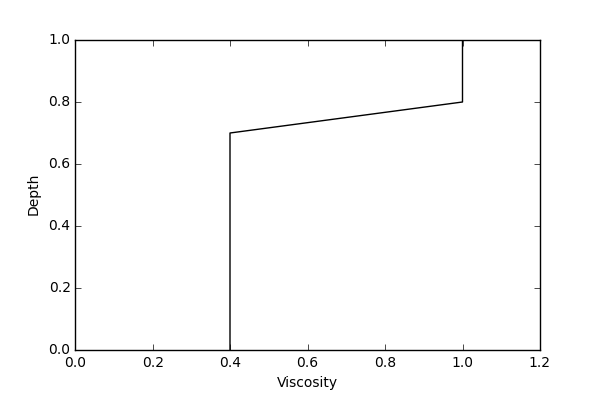
\includegraphics[width=0.25\linewidth]{cookbooks/convection-box/viscosityjumpprofile.png}
    
    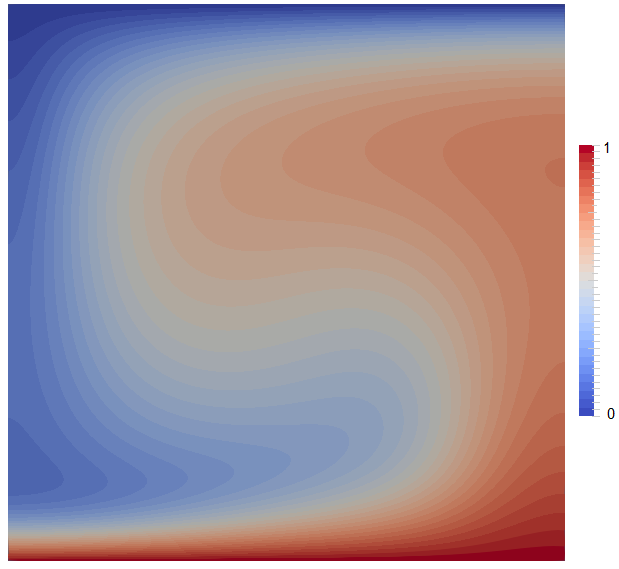
\includegraphics[width=0.3\linewidth]{cookbooks/convection-box/viscosityjumplowmodif.png}
    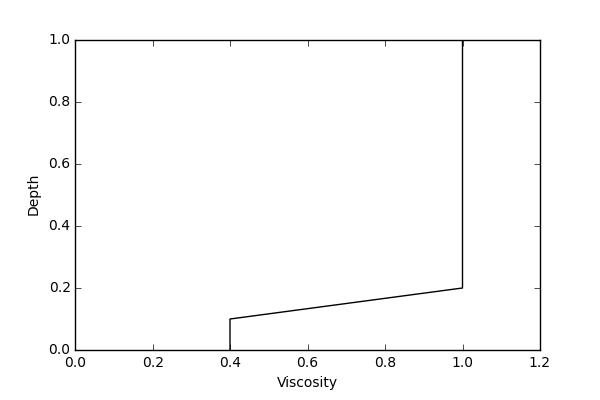
\includegraphics[width=0.25\linewidth]{cookbooks/convection-box/viscosityjumplowprofile.png}
    \caption{Convection box and the viscosity profile associated for $Ra=10^4$.}
    \label{viscosityjump}
       \end{center}
\end{figure}
\end{document}